\subsection{Тесты}
При подаче заявке важно чтобы при создании, одобрении или отклонении заявки -
заявитель был уведомлен по email о соответствующем действии (рисунок
\ref{ris:accept_reject_bid}).

\begin{figure}[h]
\center{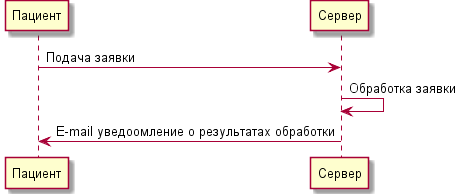
\includegraphics[width=0.7\linewidth]{accept_reject_bid.eps}}
\caption{Процесс обработки заявки}
\label{ris:accept_reject_bid}
\end{figure}

Рассмотрим тестирование процесса подачи заявки на регистрацию (листинг
\ref{lst:test_bid}).

\begin{lstlisting}[language=Ruby,caption=Тестирование подачи заявки
,label={lst:test_bid}] 
require 'spec_helper'

describe Bid do
  before { BidMailer.deliveries.clear }

  # #{Проверяем валидацию полей заявки}
  it 'should be valid' do
    # #{Создаем экземпляр заявки}
    b = build(:bid)
    # #{Проверяем верность заполнения}
    b.should be_valid
  end

  # #{Проверяем что после создания заявки, будет отослано письмо заявителю}
  it 'should send email after created' do
    # #{Создаем и сохраняем заявку в базе}
    b = create(:bid)
    # #{Проверяем что было отослано одно e-mail сообщение}
    BidMailer.deliveries.count.should eq(1)
    # #{Проверяем что адрес отправки совпадает с адресом заявителя}
    BidMailer.deliveries.last.to.should eq([b.email])
  end

  # #{Проверяем что после отклонения заявки будет отослано письмо заявителю}
  it 'should rejected' do
    # #{Создаем и сохраняем заявку в базе}
    b = create(:bid)
    BidMailer.deliveries.clear
    # #{Отклоняем заявку}
    b.reject
    # #{Проверяем что было отослано одно e-mail сообщение}
    BidMailer.deliveries.count.should eq(1)
    # #{Проверяем что адрес отправки совпадает с адресом заявителя}
    BidMailer.deliveries.last.to.should eq([b.email])
    # #{Проверяем что заявка помечена в базе как отклоненная}
    b.status.should eq('rejected')
  end

 # #{Проверяем что после одобрения заявки будет отослано письмо заявителю}
 it 'should approved' do
    # #{Создаем и сохраняем заявку в базе}
    b = create(:bid)
    BidMailer.deliveries.clear
    # #{Принимаем заявку}
    b.approve
    # #{Проверяем что было отослано одно e-mail сообщение}
    BidMailer.deliveries.count.should eq(1)
    # #{Проверяем что адрес отправки совпадает с адресом заявителя}
    BidMailer.deliveries.last.to.should eq([b.email])
    # #{Проверяем что заявка помечена в базе как принятая}
    b.status.should eq('approved')
  end
end
\end{lstlisting}

% 
% Так как в системе используются параметры разного типа нужно тестировать правила
% валидации для каждого параметра. В листинге \ref{lst:test_bool_parameter} тестируются
% возможные значения для булевого параметра.
% 
% \begin{lstlisting}[language=Ruby,caption=Тестирование возможных значений для
% булевого параметра ,label={lst:test_bool_parameter}] 
% describe BoolParameter do
%   context 'validate metadata' do
%     it 'should be valid' do
%       p = build(:bool_parameter, :metadata => {
%           :values => %w(true false),
%           :default => 'false'
%       })
%       p.should be_valid
%     end
% 
%     it 'should be invalid' do
%       p = build(:bool_parameter, :metadata => {
%           :values => '',
%           :default => ''
%       })
%       p.should_not be_valid
%       p.errors[:metadata].should include('parameter.bool.metadata.errors.default')
%       p.errors[:metadata].should include('parameter.bool.metadata.errors.values')
%     end
%   end
% 
%   context 'validate value' do
%     before(:each) do
%       @pr = build(:bool_parameter)
%     end
% 
%     it 'should be valid' do
%       @pr.validate_value(true).should eq(true)
%       @pr.validate_value(false).should eq(true)
%       @pr.validate_value('true').should eq(true)
%       @pr.validate_value('false').should eq(true)
%     end
% 
%     it 'should be not valid' do
%       @pr.validate_value(Class).should eq(false)
%       @pr.validate_value(123).should eq(false)
%     end
%   end
% end
% \end{lstlisting}
% 
% Более сложными тесты проверяют правильность обработки событий в системе.
% Например событие нельзя сразу перевести и статуса free в close, так как
% нарушается очередность состояний события. Тесты для проверки событий приведены в
% приложении \ref{app:events_tests}.
